\documentclass[UTF8,a4paper,12pt]{ctexart}
\usepackage[a4paper,margin=2.35cm]{geometry}
\usepackage{amsmath,amssymb,bm}
\usepackage{booktabs,multirow,array,makecell,longtable}
\usepackage{graphicx,float,subcaption}
\usepackage{xcolor,hyperref,enumitem,caption}
\usepackage{listings}
\hypersetup{colorlinks=true,linkcolor=blue,citecolor=blue,urlcolor=blue}
\graphicspath{{results/figures/}}
\setlength{\parindent}{2em}
\setlength{\parskip}{0.25em}
\captionsetup{font=small,labelfont=bf}
\lstset{basicstyle=\ttfamily\small,breaklines=true,frame=single,columns=fullflexible,showstringspaces=false}

\title{基于重复测量模型与风险约束分类的\quad NIPT时点选择与胎儿异常判定}
\author{数学建模分析报告}
\date{\today}

\begin{document}
\maketitle
\begin{center}
\textbf{摘要}
\end{center}

无创产前检测（NIPT）的有效性同时受到检测孕周、孕妇 BMI、个体差异以及测序质量的影响。本文以附件中的男胎检测记录和女胎检测记录为基础，首先统一孕周格式、保留同一孕妇的重复检测，并按孕妇层级进行统计建模。针对问题一，在 Y 染色体浓度的 logit 空间建立含孕妇随机截距的重复测量模型；模型在原浓度尺度上的 $R^2$ 为 $0.811$，RMSE 为 $0.0146$，孕周二次项显著（$p=4.23\times 10^{-14}$），孕周相关项的似然比检验显著（$p=3.68\times10^{-14}$）。

针对问题二，将男胎孕妇按 BMI 的有序动态规划分组，并以达标概率的置信下界为安全约束。数据驱动得到两个区间：$BMI<36.78$ 与 $BMI\ge36.78$。前者推荐在 $22.5$ 周检测，模型预测达标概率为 $0.958$；后者在观测窗口内推荐 $25.0$ 周检测，但置信下界尚未达到 $0.90$，应采用复检和加强监测策略。针对问题三，进一步引入年龄、身高、体重、孕产史、测序质量和 IVF 状态，在问题二安全时点基础上构造综合风险函数。两组的风险受安全下限约束后均在 $25.0$ 周达到最小，预测达标比例分别为 $0.935$ 和 $0.793$，说明高 BMI 组不宜仅依靠一次检测作出结论。

针对问题四，将女胎非整倍体字段非空定义为异常，以 Z 值、X 染色体信息、GC 含量、读段质量和孕妇特征为输入，比较 Z 值阈值、带类别权重的 Logistic 回归和随机森林。按孕妇分组的交叉验证表明，Logistic 回归 ROC-AUC 为 $0.812$，在灵敏度约 $0.90$ 的阈值下样本级灵敏度为 $0.925$；随机森林 ROC-AUC 为 $0.768$。传统“任一 Z 值绝对值超过 3”规则的灵敏度仅为 $0.060$，不能单独作为本数据集的最终判定器。综合结果支持“先以模型筛查，再以复检和临床诊断确认”的判定流程。

\noindent\textbf{关键词：} NIPT；重复测量；BMI 分组；达标概率；Logistic 回归；非整倍体判定

\section{问题重述}

NIPT 通过检测母体血液中的胎儿游离 DNA 判断染色体异常。胎儿 DNA 在母体血浆中的发现为无创检测提供了分子基础\cite{Lo1997}，大规模平行测序已被用于常见染色体非整倍体筛查\cite{Chiu2011,Bianchi2014}。男胎样本的 Y 染色体浓度随孕周和孕妇身体特征变化，达到 $4\%$ 是保证检测可靠性的经验标准；女胎不含 Y 染色体，需要利用 13、18、21 号染色体的 Z 值、X 染色体信息和测序质量指标综合判断异常。

本文需解决四个相互衔接的问题：
\begin{enumerate}[label=(\arabic*),leftmargin=3em]
  \item 分析 Y 染色体浓度与孕周、BMI 及其他指标的关系，并检验显著性；
  \item 仅依据 BMI 对男胎孕妇合理分组，给出达到 $4\%$ 的最佳检测时点；
  \item 综合年龄、身高、体重、孕产史、测序误差和达标比例，重新确定分组和检测时点；
  \item 针对女胎建立异常判定模型，兼顾漏诊和误诊风险。
\end{enumerate}

\section{问题分析与总体流程}

问题一是带有重复观测的非线性回归问题。同一孕妇通常有 4 次左右检测，若直接把所有记录当作独立样本，会低估标准误，因此使用孕妇随机截距模型；随机效应模型是纵向数据分析的经典工具\cite{Laird1982}。问题二是带有临床安全约束的有序分组问题，BMI 分组必须保持区间连续，分组数量过多会造成高 BMI 小样本组不稳定。问题三在问题二的基础上引入个体化特征，并把测量误差和延迟检测风险纳入目标函数\cite{Fuller1987}。问题四是类别不平衡的二分类问题，异常样本仅占 67/605，评价时必须同时报告 ROC-AUC、PR-AUC、灵敏度和特异度。

本文的总体数据流为：
\begin{center}
数据清洗与孕周解析 $\rightarrow$ 问题一重复测量回归 $\rightarrow$ BMI 有序分组与安全时点 $\rightarrow$ 多因素风险优化 $\rightarrow$ 女胎异常分类与复检规则。
\end{center}

\begin{figure}[H]
  \centering
  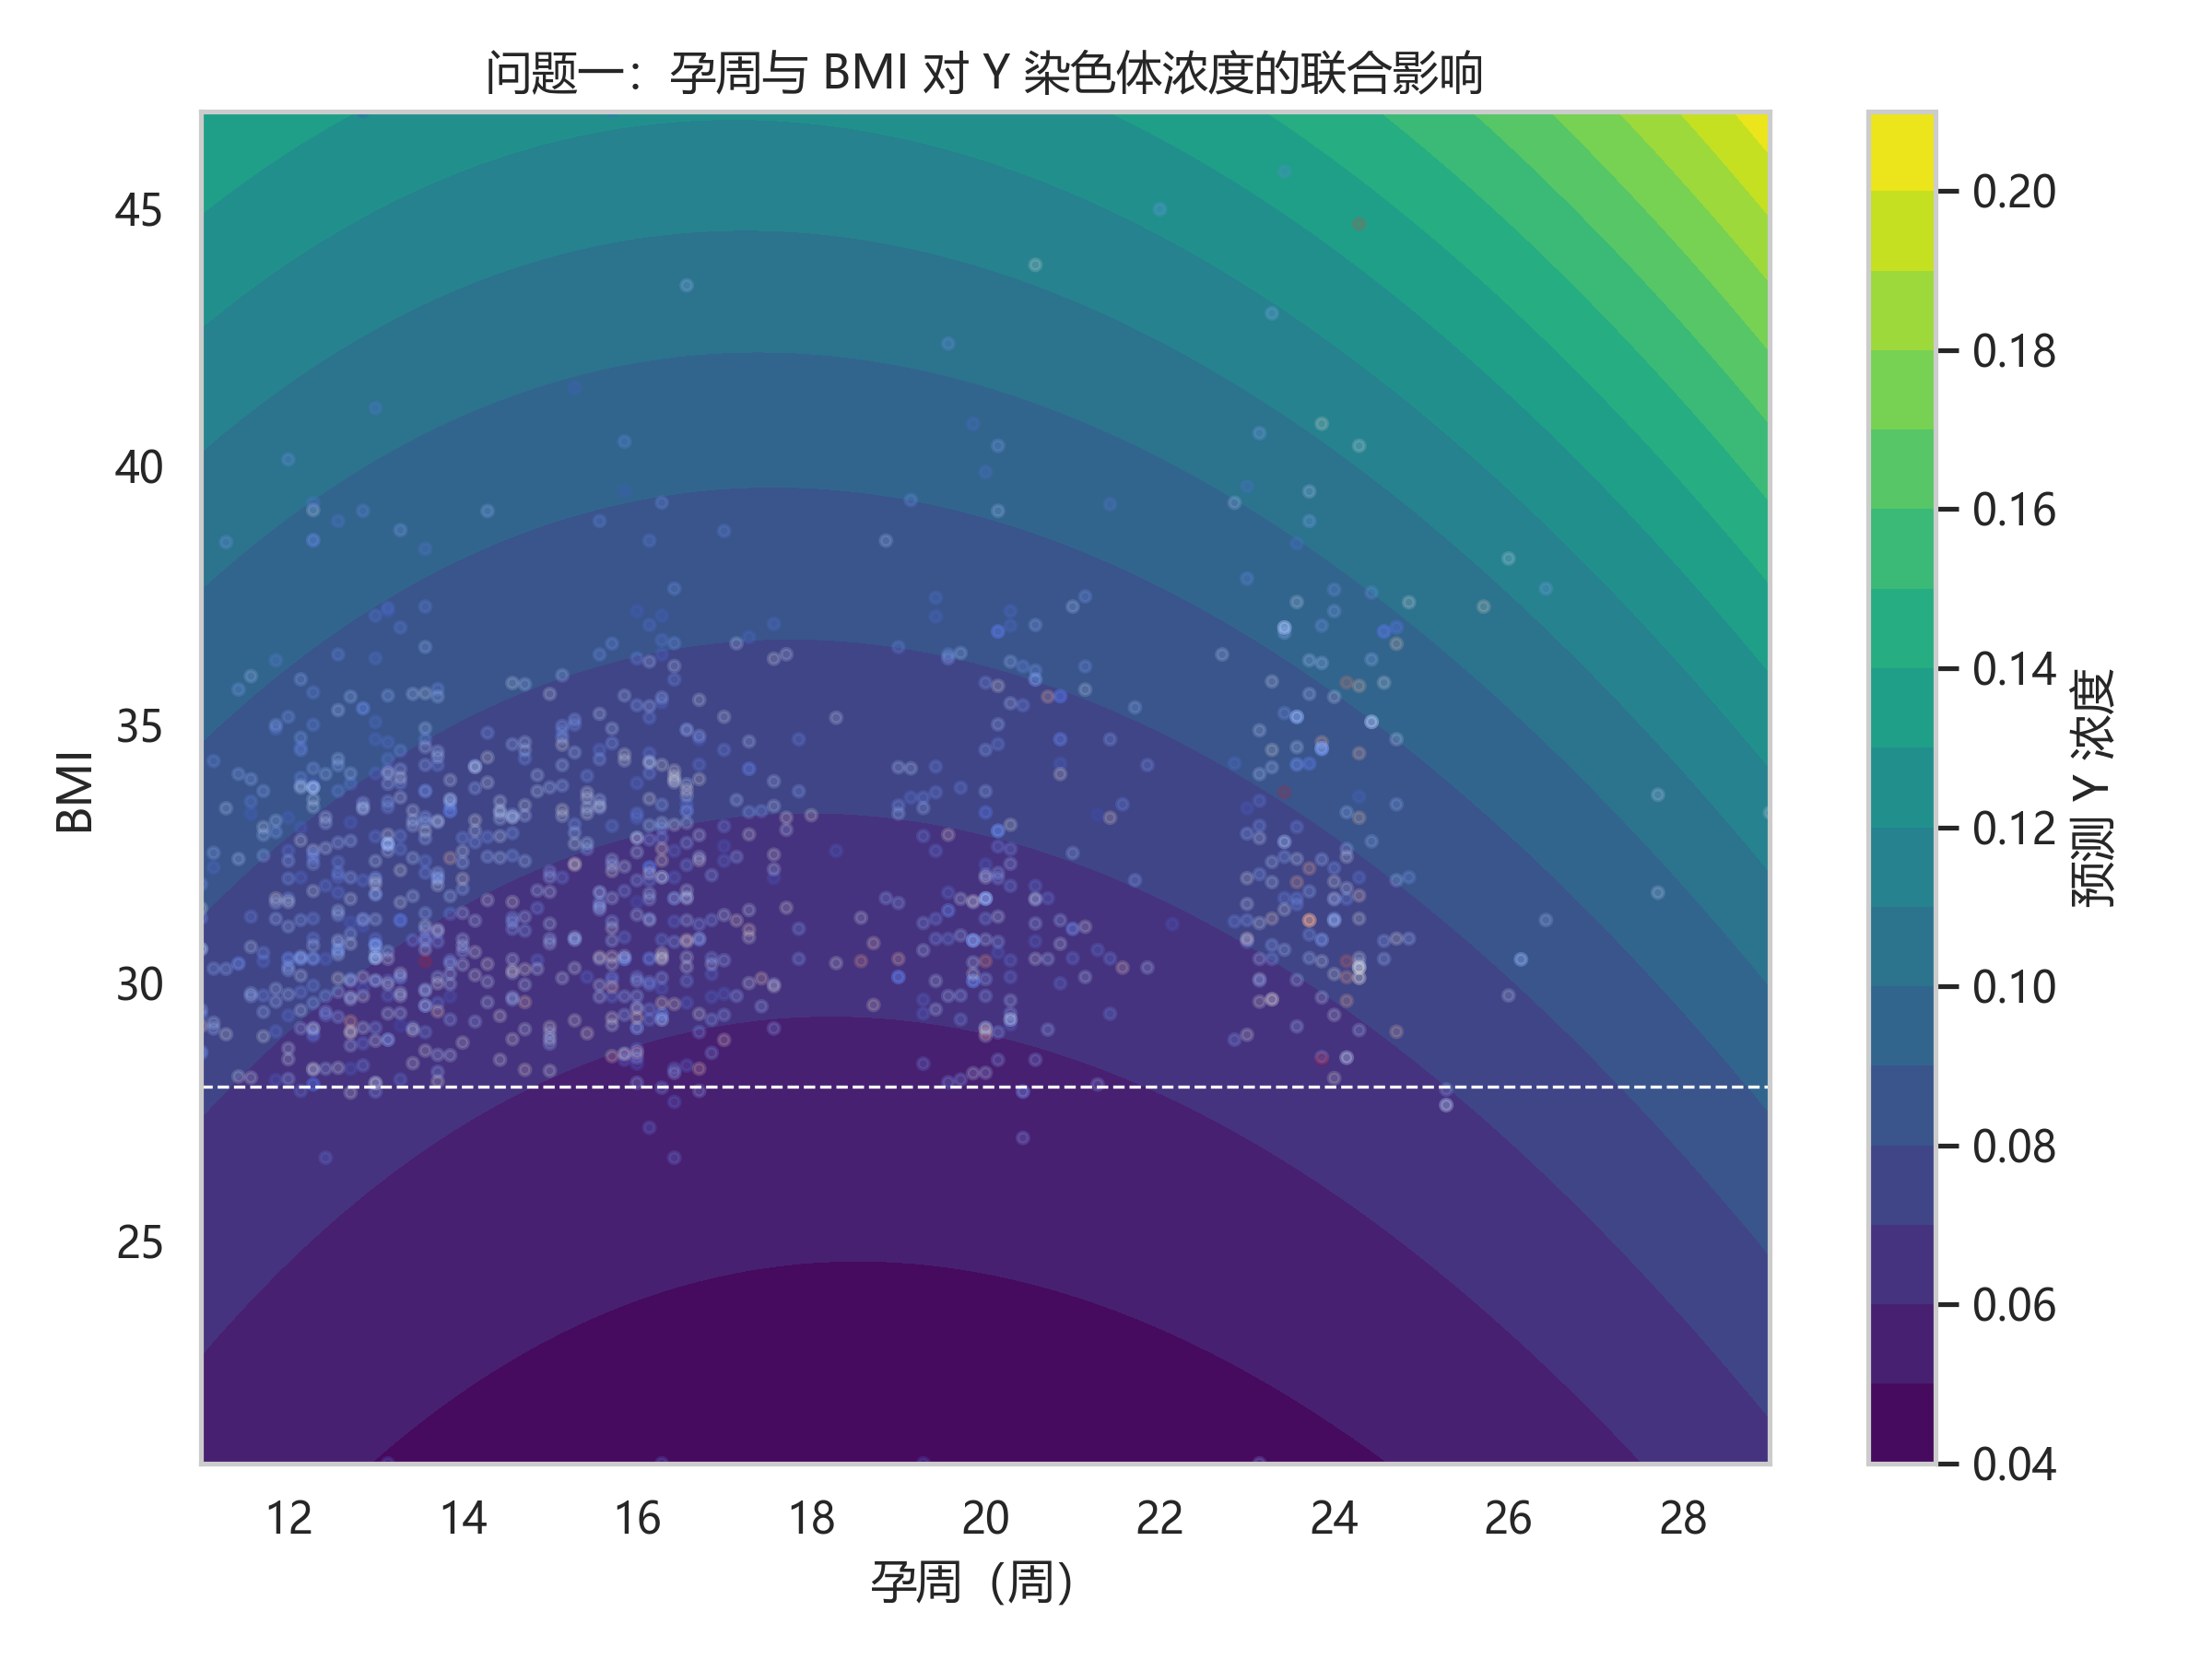
\includegraphics[width=0.92\textwidth]{q1_week_bmi_surface.png}
  \caption{孕周与 BMI 对男胎 Y 染色体浓度的联合影响}
\end{figure}

\section{数据处理、符号与假设}

\subsection{数据概况}

男胎数据包含 1082 条检测记录、267 位孕妇，其中 260 位有重复检测，最多一位孕妇有 8 次检测；女胎数据包含 605 条记录、147 位孕妇，其中 143 位有重复检测，女胎异常标签为 67 条记录。孕周字段统一解析为周数小数，例如 $11w+6$ 转为 $11+6/7$。

\begin{table}[H]
\centering
\caption{数据审计结果}
\begin{tabular}{lrrrrr}
\toprule
数据集 & 记录数 & 孕妇数 & 重复孕妇数 & 最大检测次数 & 异常记录数\\
\midrule
男胎 & 1082 & 267 & 260 & 8 & --\\
女胎 & 605 & 147 & 143 & 9 & 67\\
\bottomrule
\end{tabular}
\end{table}

\subsection{清洗与质量控制}

对读段数、比对比例、重复比例、GC 含量和过滤比例进行数值化。对建模所需连续变量采用中位数填补缺失值；孕妇代码作为分组变量保留，不将重复检测简单删除。女胎文件中两个空的导出列不参与建模。GC 含量偏离 $[0.40,0.60]$、比对比例低于 $0.70$ 或过滤比例高于 $0.05$ 的记录被标记为质量风险，但不在主分析中直接删除，以便在误差分析中评估质量因素的影响。

\subsection{符号说明与建模假设}

\begin{table}[H]
\centering
\caption{主要符号}
\begin{tabular}{>{\centering\arraybackslash}p{0.18\textwidth}p{0.60\textwidth}p{0.12\textwidth}}
\toprule
符号 & 含义 & 单位\\
\midrule
$w_{ij}$ & 第 $i$ 位孕妇第 $j$ 次检测的孕周 & 周\\
$B_i$ & 第 $i$ 位孕妇 BMI & 无量纲\\
$Y_{ij}$ & 男胎 Y 染色体浓度 & 比例\\
$A_{ij}$ & 是否达到 $Y_{ij}\ge0.04$ & 0/1\\
$b_i$ & 孕妇随机截距 & logit尺度\\
$p_i(t)$ & 个体在孕周 $t$ 达标的概率 & 比例\\
$Z_{13},Z_{18},Z_{21}$ & 三条常见染色体 Z 值 & 无量纲\\
\bottomrule
\end{tabular}
\end{table}

作如下假设：
\begin{enumerate}[label=H\arabic*.,leftmargin=3em]
  \item 同一孕妇的多次检测共享一个稳定的个体随机截距，剩余误差在 logit 空间近似服从正态分布；
  \item $Y=0.04$ 是题目给出的男胎检测可靠性阈值，推荐时点必须先满足达标概率约束，再比较孕周；
  \item 对于从未观测到达标的孕妇，其首次达标时间是右删失的，分组优化时使用最后观测孕周加 1 周作为保守代理，不把它误认为已经达标；
  \item 女胎异常标签以附件的非整倍体字段为监督标签，模型输出是筛查建议而非临床诊断结论。
\end{enumerate}

\section{问题一：Y 染色体浓度关系模型}

\subsection{模型建立}

由于浓度是 $(0,1)$ 内的比例，先进行 logit 变换。Logistic 链接函数及其估计方法参见广义线性模型框架\cite{McCullagh1989,Hosmer2013}：
\begin{equation}
  L_{ij}=\log\frac{Y_{ij}}{1-Y_{ij}}.
\end{equation}
对孕周、BMI 及连续协变量作稳健中心化，建立随机截距模型：
\begin{equation}
\begin{aligned}
L_{ij}={}&\beta_0+\beta_1 w_{ij}+\beta_2 w_{ij}^2+\beta_3 B_i+\beta_4 B_i^2+\beta_5w_{ij}B_i\\
&+\gamma_1 Age_i+\gamma_2 Height_i+\gamma_3 Weight_i+\gamma_4 Draw_{ij}\\
&+\gamma_5\log(Reads_{ij}+1)+\gamma_6 Map_{ij}+\gamma_7 Dup_{ij}+\gamma_8GC_{ij}+\gamma_9Filter_{ij}+b_i+\varepsilon_{ij},
\end{aligned}
\end{equation}
其中 $b_i\sim N(0,\sigma_b^2)$。孕周二次项允许浓度随孕周呈弯曲关系；交互项用于检验 BMI 是否改变孕周效应。

\subsection{相关性与显著性}

Spearman 相关分析中，Y 浓度与体重、BMI、年龄、身高的相关系数分别为 $-0.167$、$-0.155$、$-0.117$ 和 $-0.101$；与孕周的单调相关系数为 $0.084$。这些系数绝对值不大，说明个体差异和检测批次因素不可忽略，因此不宜只用单变量线性回归。

\begin{table}[H]
\centering
\caption{问题一模型的主要参数与显著性}
\resizebox{\textwidth}{!}{%
\begin{tabular}{lrrrr}
\toprule
变量 & 系数 & 标准误 & $p$值 & 解释\\
\midrule
$w$ & $-0.0834$ & 0.0297 & 0.0049 & 线性孕周项\\
$w^2$ & $0.0898$ & 0.0119 & $4.23\times10^{-14}$ & 非线性孕周项\\
$B$ & 0.1070 & 0.2307 & 0.6429 & BMI一次项\\
$B^2$ & 0.0011 & 0.0078 & 0.8902 & BMI二次项\\
$wB$ & 0.0068 & 0.0087 & 0.4321 & 孕周--BMI交互项\\
$Draw$ & 0.2416 & 0.0258 & $8.15\times10^{-21}$ & 抽血次数\\
$\log(Reads+1)$ & $-0.2102$ & 0.0456 & $4.01\times10^{-6}$ & 读段规模\\
$GC$ & 6.7008 & 2.7911 & 0.0164 & 总体 GC 含量\\
\bottomrule
\end{tabular}}
\end{table}

模型在原始浓度尺度上的 $R^2=0.811$，RMSE 为 $0.0146$，MAE 为 $0.0101$；孕妇随机截距方差为 $2.187$，说明同一孕妇间存在显著的稳定差异。似然比检验表明，去掉孕周项后 $\chi^2=65.63$、$p=3.68\times10^{-14}$；去掉 BMI 项后 $p=0.818$；去掉交互项后 $p=0.432$。因此，本数据中孕周的非线性作用明确，BMI 的独立线性作用和与孕周的交互项没有达到显著水平，但 BMI 仍适合在时点优化中作为分组变量。

\begin{figure}[H]
\centering
\begin{subfigure}{0.48\textwidth}
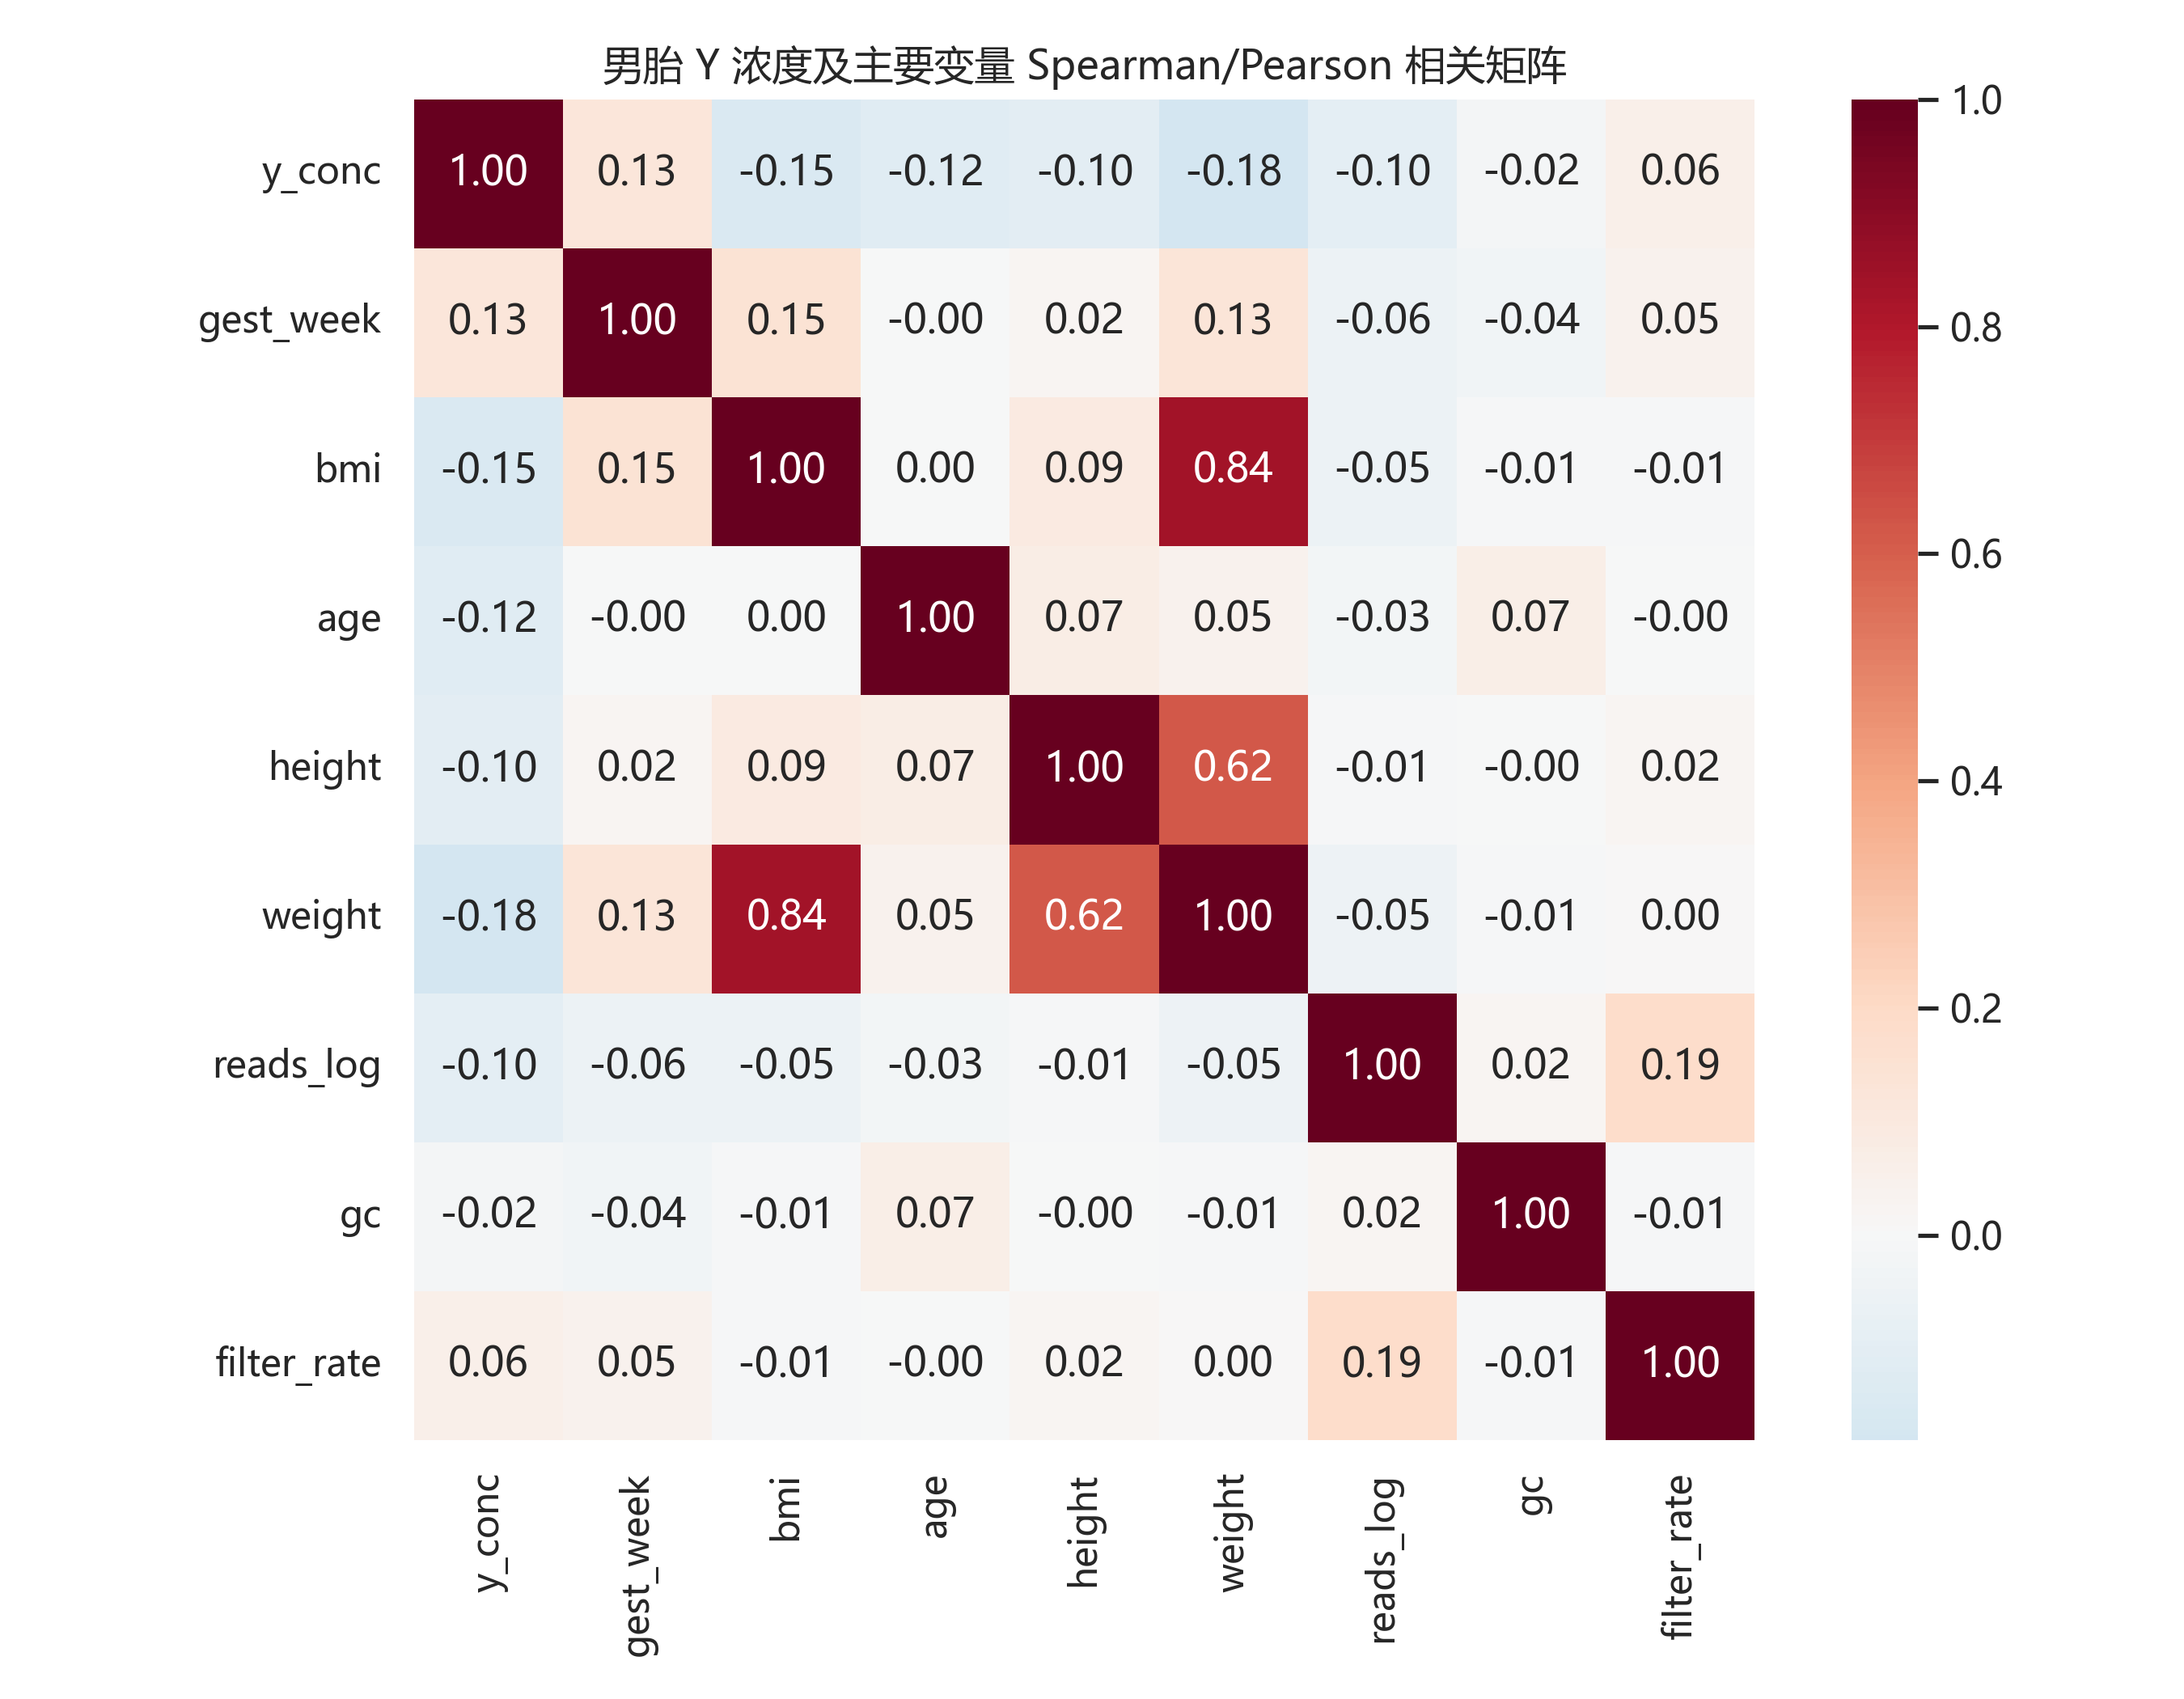
\includegraphics[width=\textwidth]{q1_correlation_heatmap.png}
\caption{相关矩阵}
\end{subfigure}
\begin{subfigure}{0.48\textwidth}
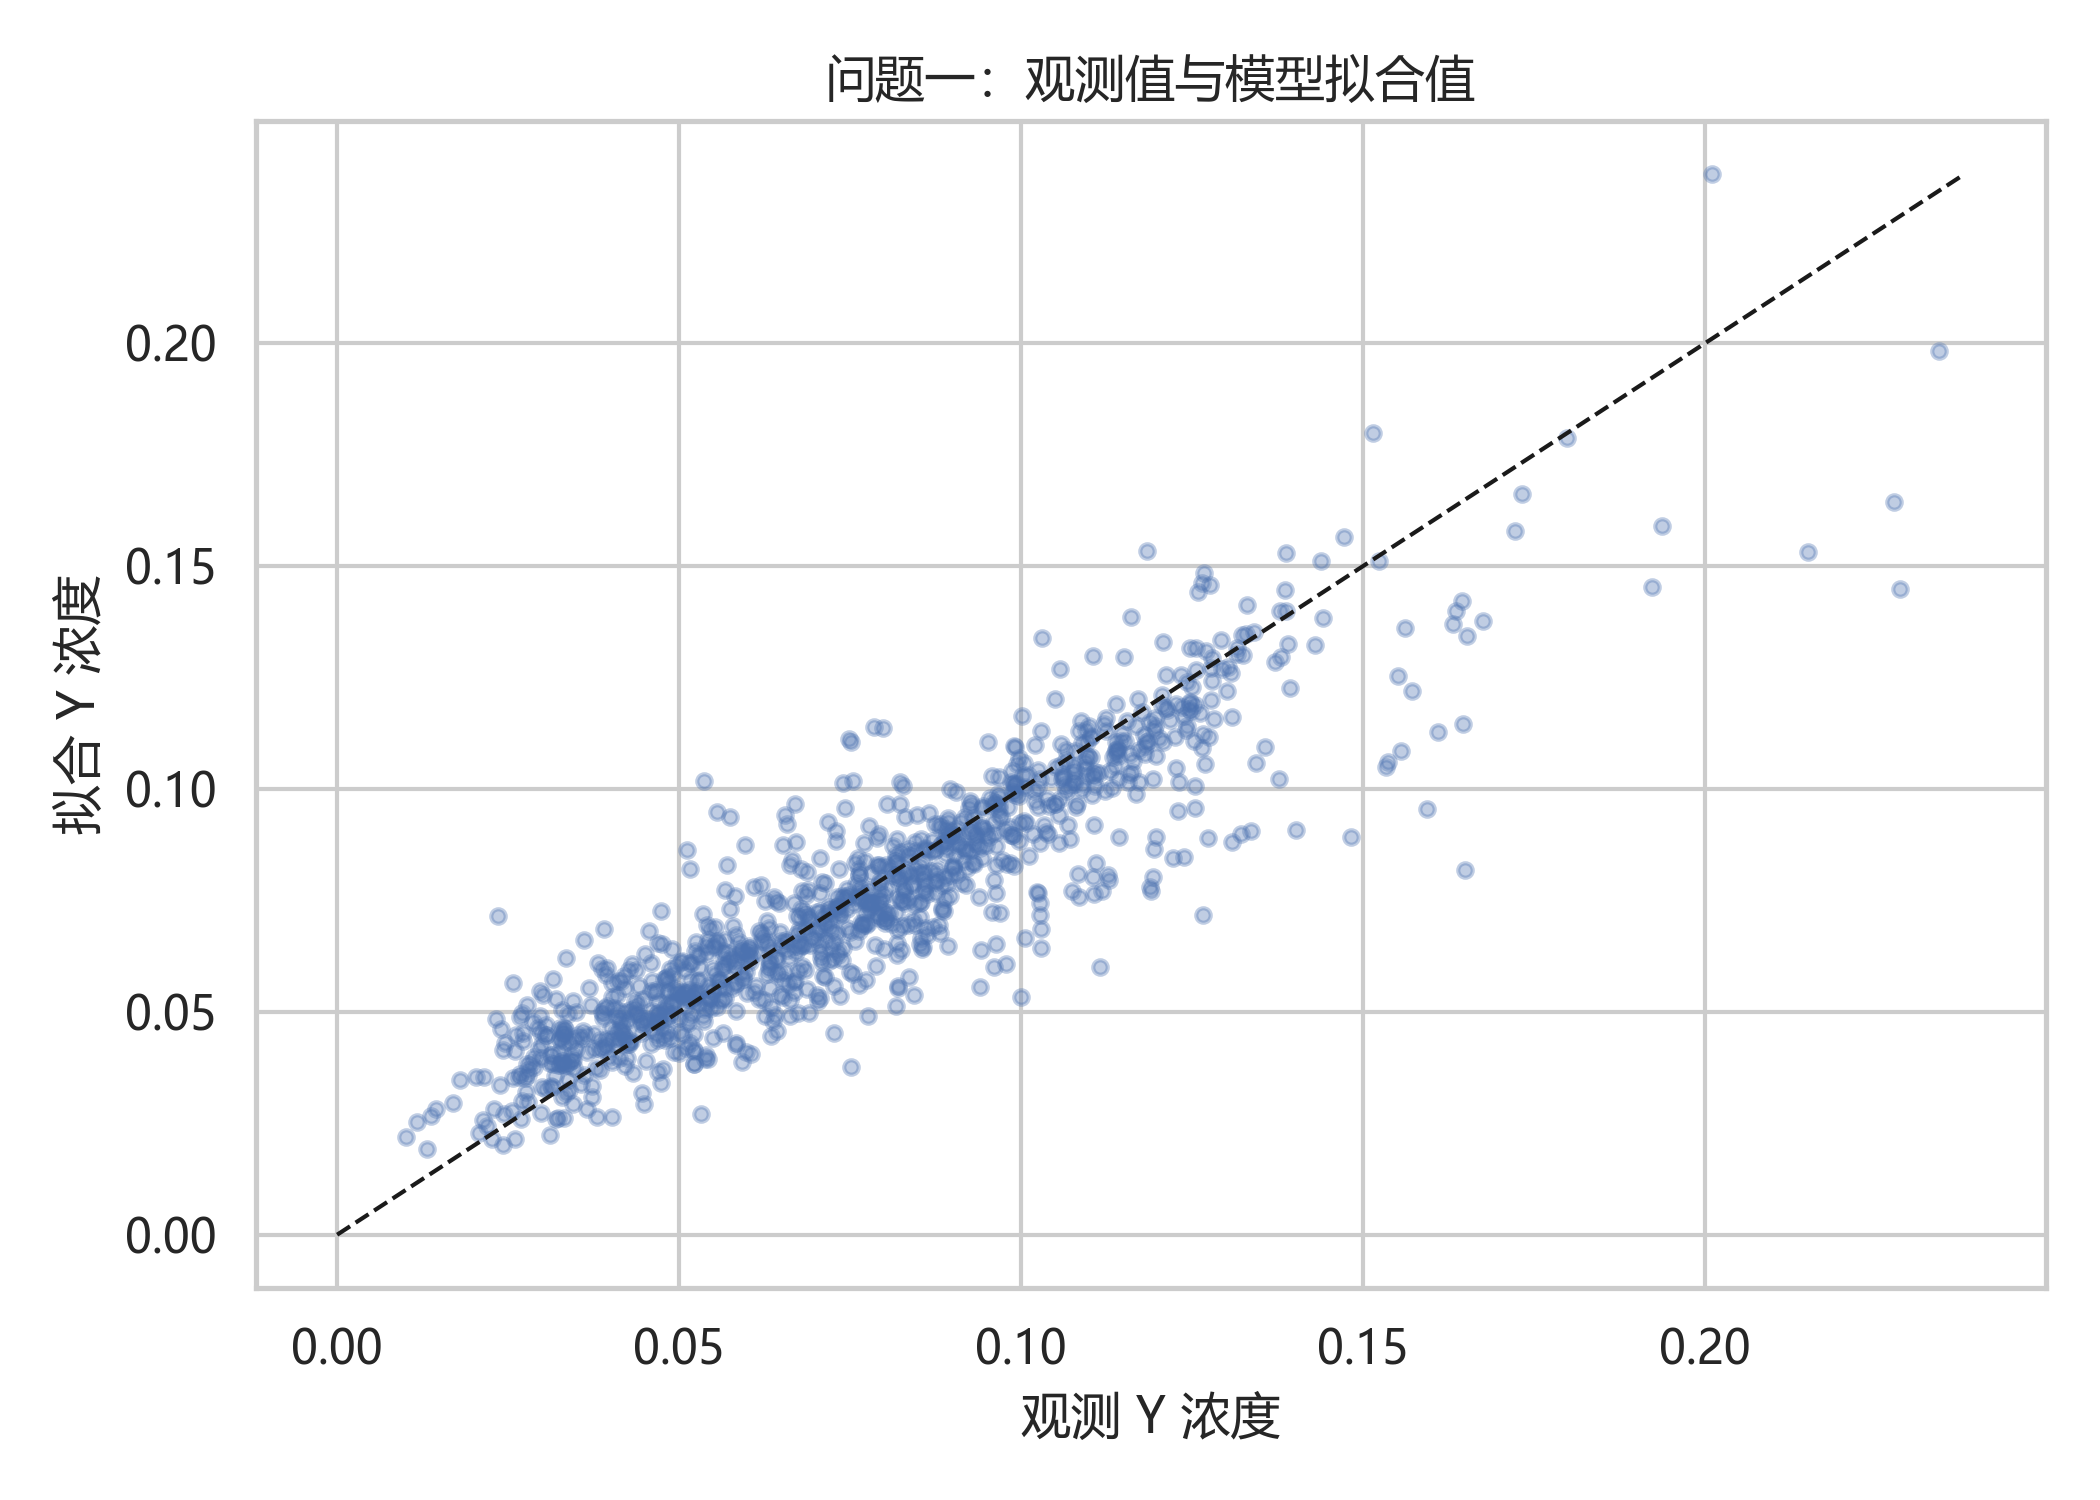
\includegraphics[width=\textwidth]{q1_observed_fitted.png}
\caption{观测值与拟合值}
\end{subfigure}
\caption{问题一模型诊断图}
\end{figure}

\section{问题二：基于 BMI 的分组与最佳 NIPT 时点}

\subsection{达标概率模型}

定义 $A_{ij}=I(Y_{ij}\ge0.04)$，采用带孕妇聚类稳健标准误的 Logistic GEE/GLM 模型：
\begin{equation}
\operatorname{logit}\{P(A_{ij}=1)\}=\alpha_0+\alpha_1w_{ij}+\alpha_2w_{ij}^2+\alpha_3B_i+\alpha_4w_{ij}B_i.
\end{equation}
该模型的孕周一次项、二次项 $p$ 值分别为 $0.0127$ 和 $0.0178$，BMI 一次项 $p=0.2658$，交互项 $p=0.7944$。因此推荐时点主要由孕周驱动，而 BMI 的作用更适合通过分组后对高 BMI 人群进行风险控制。

\subsection{BMI 有序分组}

以每位孕妇的首次达标时间为目标，对 BMI 排序后采用连续区间动态规划。目标函数为组内保守达标时间平方离差加组数惩罚：
\begin{equation}
  \min_{\mathcal{G}}\sum_{g\in\mathcal{G}}\sum_{i\in g}(\tilde t_i-\bar t_g)^2+\lambda |\mathcal{G}|\log n,
\end{equation}
其中 $\tilde t_i$ 为首次达标时间或右删失代理。候选组数为 2--5，每组至少保留 18 位孕妇。最优分组为：
\begin{table}[H]
\centering
\caption{问题二 BMI 分组与推荐时点}
\begin{tabular}{lrrrrrr}
\toprule
组别 & BMI 区间 & 孕妇数 & 首次达标中位数 & 推荐孕周 & 预测达标率 & 置信下界\\
\midrule
1 & $(-\infty,36.78)$ & 248 & 12.71 & 22.5 & 0.958 & 0.900\\
2 & $[36.78,+\infty)$ & 19 & 15.86 & 25.0 & 0.971 & 0.779\\
\bottomrule
\end{tabular}
\end{table}

时点定义为在候选孕周中最早满足预测达标概率置信下界约束的时点。第一组在 $22.5$ 周达到下界 $0.900$，第二组在 25 周时点预测概率较高但区间仍较宽，原因是高 BMI 组样本仅 19 位孕妇。因此，第二组不能简单解释为“25 周检测即可保证准确”，更合理的临床策略是 25 周前后复检并结合其他质量指标。

\begin{figure}[H]
\centering
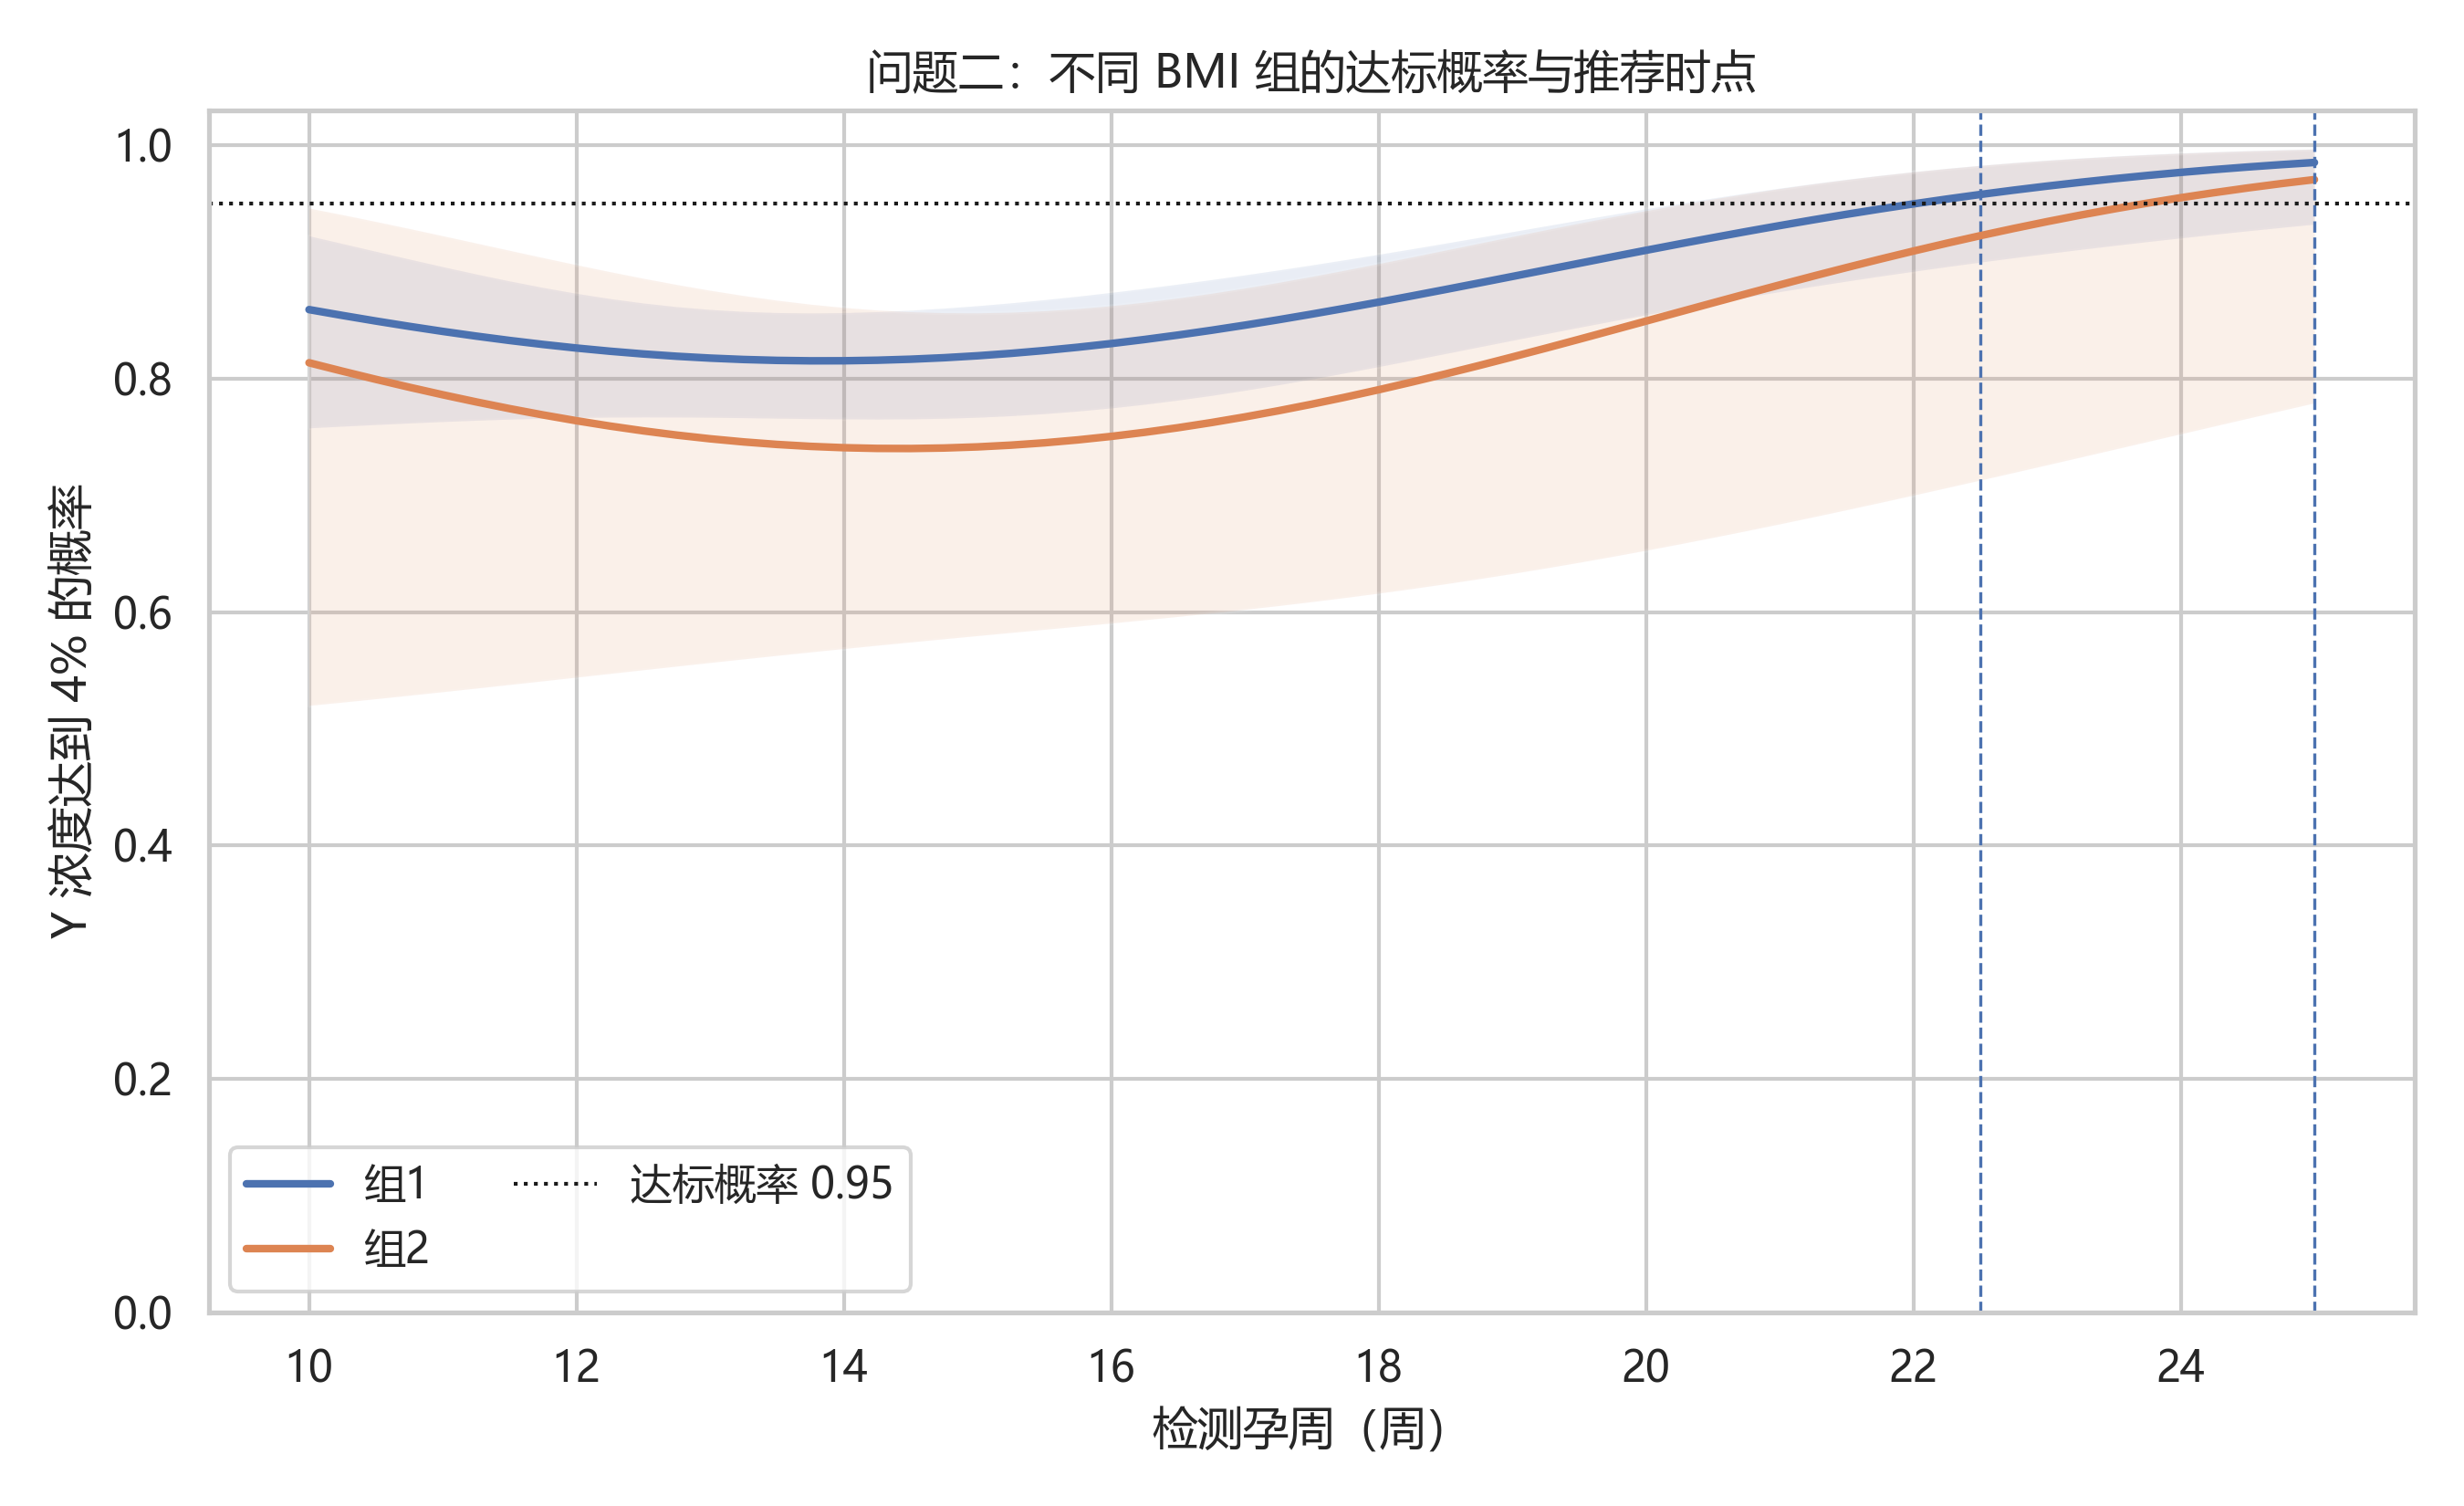
\includegraphics[width=0.82\textwidth]{q2_bmi_probability.png}
\caption{不同 BMI 组随孕周变化的 Y 浓度达标概率}
\end{figure}

\subsection{检测误差分析}

问题一模型的 logit 残差标准差为 $0.223$。在推荐时点附近对 logit 达标概率加入正态扰动并重复 3000 次，得到测量误差后的达标率和误判概率，明细保存在结果表中。误差模拟显示，第一组在推荐时点的达标概率仍约为 $0.96$；第二组的区间明显更宽，表明高 BMI 人群的关键风险不是简单的平均浓度偏移，而是个体间异质性导致的置信区间扩张。

\section{问题三：综合个体因素与检测误差的风险优化}

\subsection{多因素达标模型}

在问题二模型基础上，加入年龄、身高、体重、孕产次数、抽血次数、读段数、比对质量、重复率、GC 含量、过滤比例和 IVF 状态：
\begin{equation}
\begin{aligned}
\operatorname{logit}\{p_i(t)\}={}&\theta_0+\theta_1t+\theta_2t^2+\theta_3B_i+\theta_4tB_i\\
&+\theta_5Age_i+\theta_6Height_i+\theta_7Weight_i+\theta_8Gravidity_i+\theta_9Parity_i\\
&+\theta_{10}\log(Reads_i+1)+\theta_{11}Map_i+\theta_{12}Dup_i\\
&+\theta_{13}GC_i+\theta_{14}Filter_i+\theta_{15}IVF_i.
\end{aligned}
\end{equation}

\subsection{风险函数与安全下限}

若只最小化延迟孕周，模型可能利用少量早期记录把时点推到 10 周，忽略“过早检测导致不可靠”的题目约束。因此，问题三显式继承问题二的安全下限 $t_g^{(2)}$，并定义：
\begin{equation}
R_g(t)=4[1-\bar p_g^{err}(t)]+C(t),\qquad t\ge t_g^{(2)},
\end{equation}
其中 $\bar p_g^{err}(t)$ 为对组内真实个体特征进行 Monte Carlo 积分并加入 logit 测量扰动后的平均达标率，$C(t)$ 是孕周风险惩罚：12 周以内取 0.15，13--27 周取 0.85，28 周以后取 2.80。系数 4 用于使一次明显的准确性损失大于同组内的少量孕周移动。

\begin{table}[H]
\centering
\caption{问题三综合风险优化结果}
\begin{tabular}{lrrrrrr}
\toprule
组别 & BMI 区间 & 记录数 & 孕妇数 & 推荐孕周 & 达标比例 & 风险分数\\
\midrule
1 & $(-\infty,36.78)$ & 1000 & 254 & 25.0 & 0.935 & 1.109\\
2 & $[36.78,+\infty)$ & 82 & 27 & 25.0 & 0.793 & 1.678\\
\bottomrule
\end{tabular}
\end{table}

\begin{figure}[H]
\centering
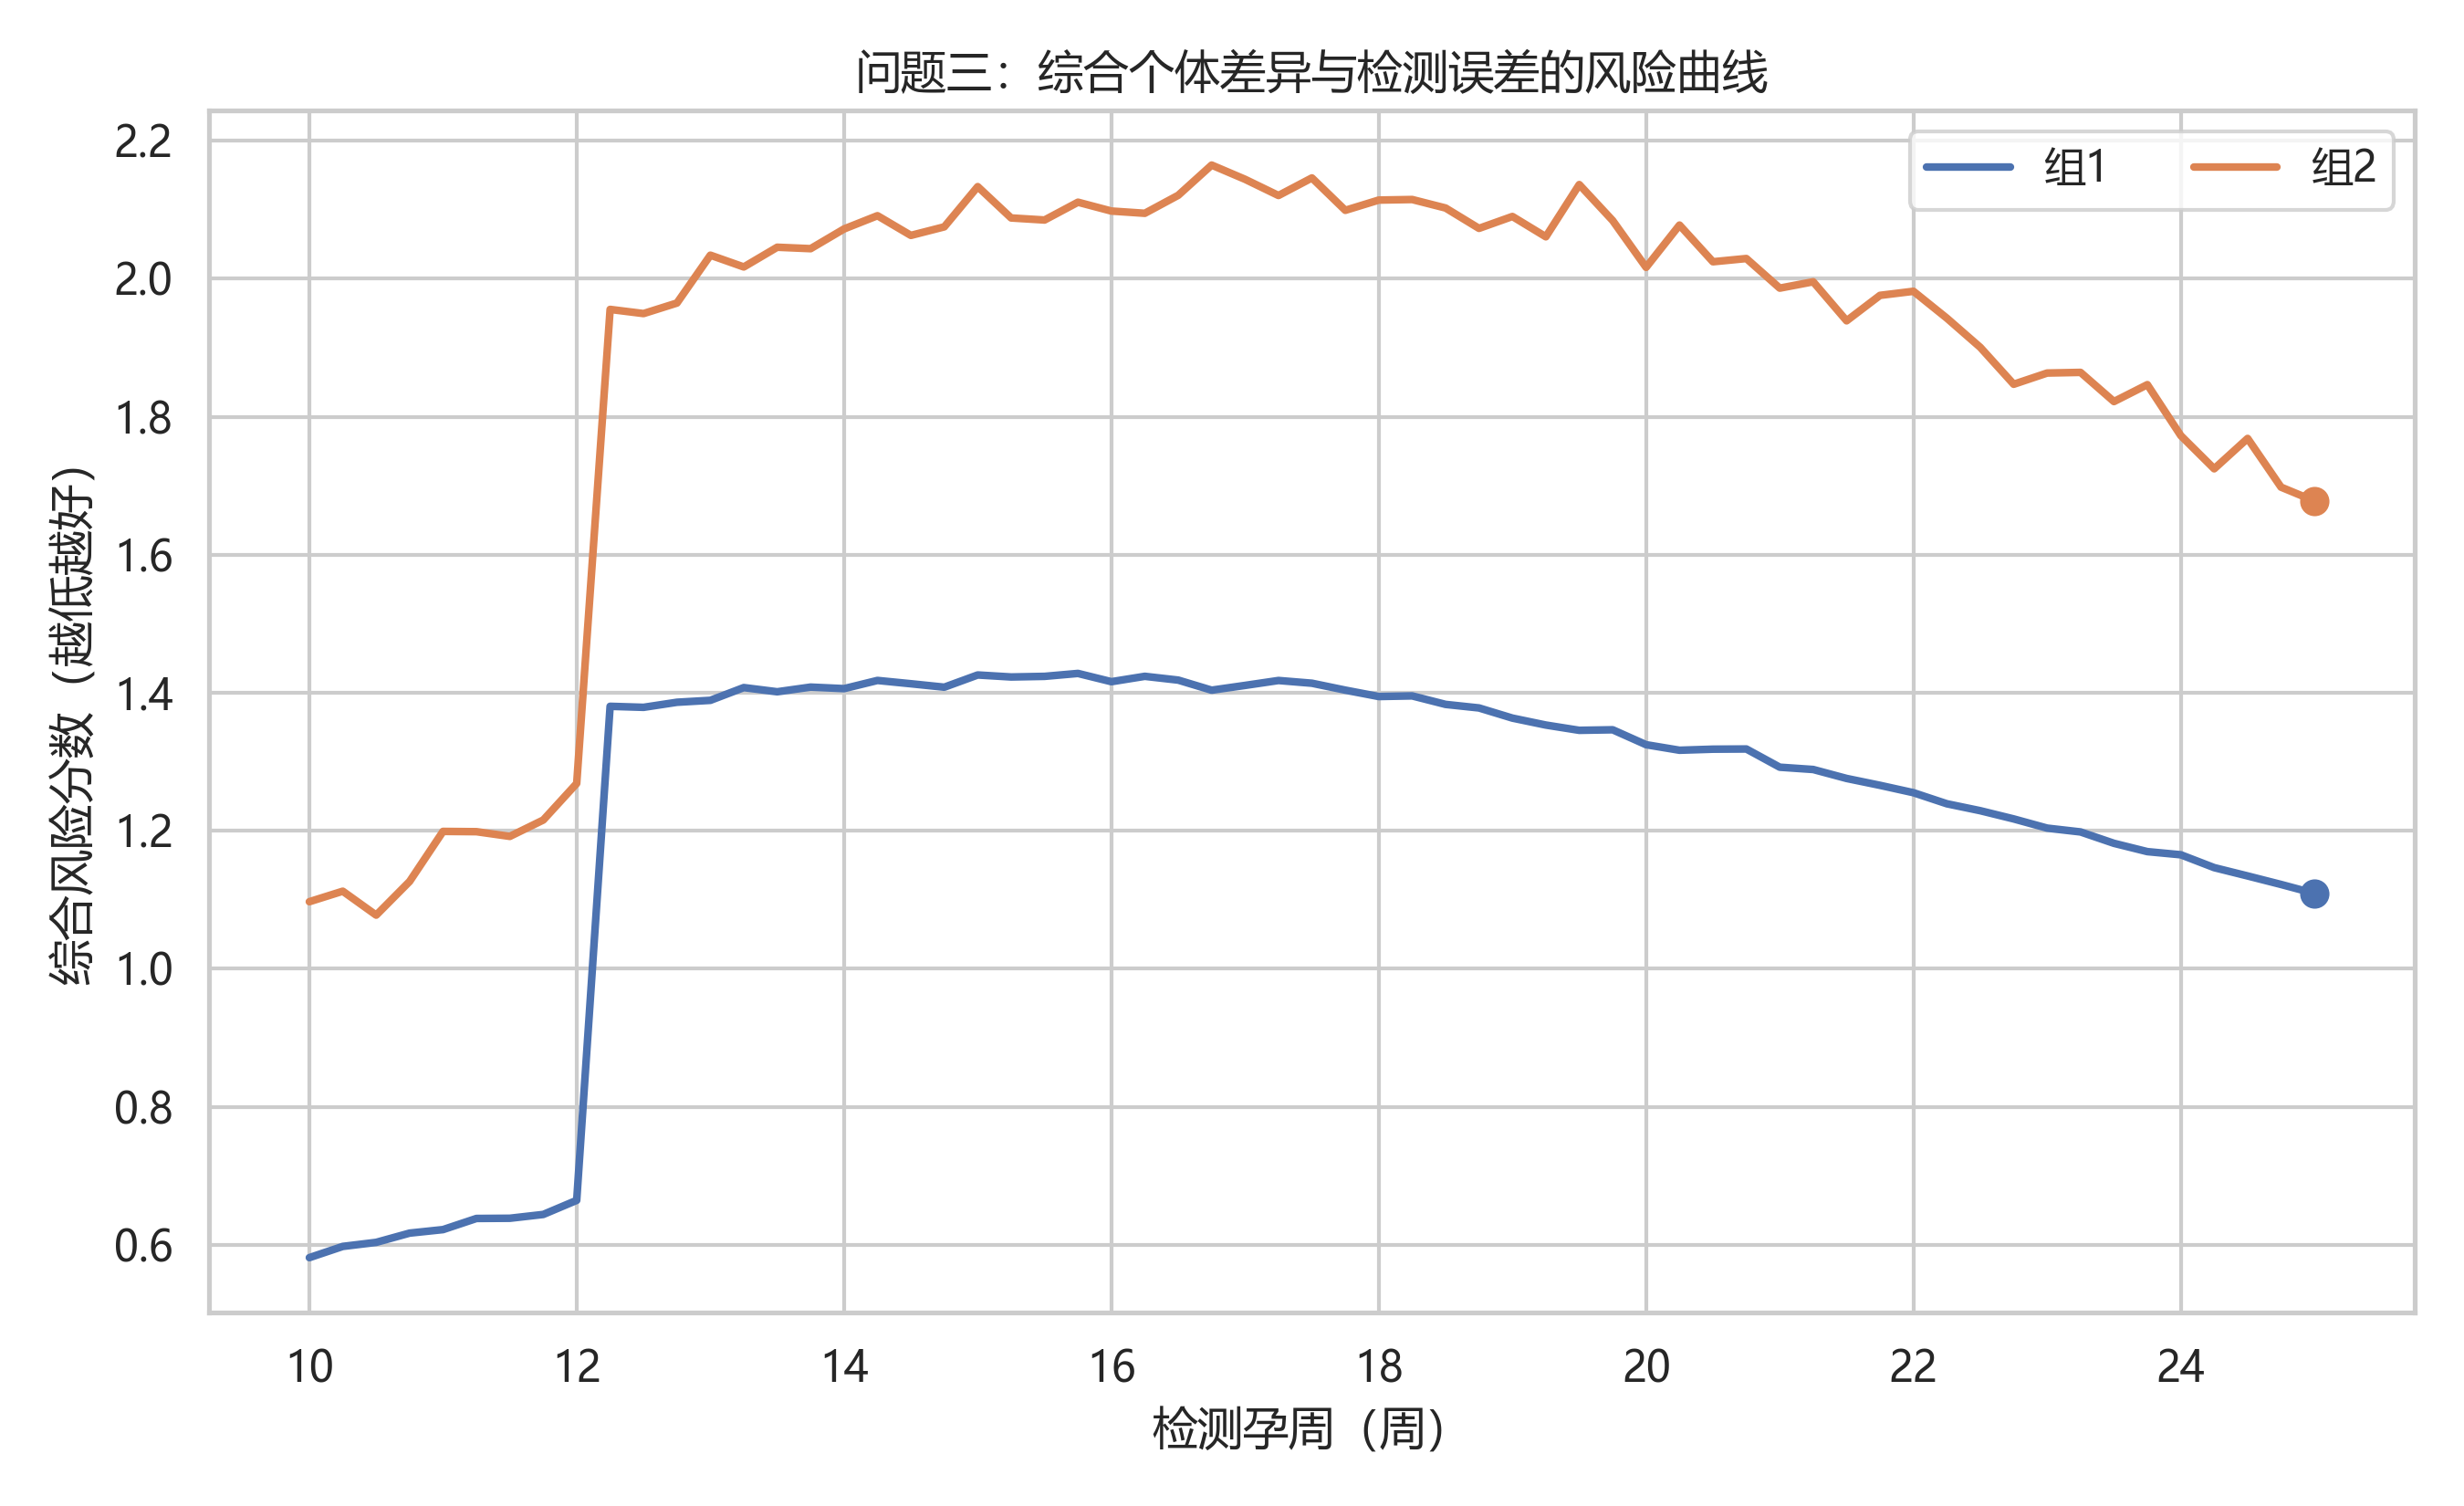
\includegraphics[width=0.82\textwidth]{q3_risk_curve.png}
\caption{综合风险曲线及推荐时点}
\end{figure}

高 BMI 组在 25 周时的预测达标比例仍只有约 $0.793$，且组内样本量小。这个结果不能被解读为“检测越晚越好”，而应解读为：在给定数据覆盖范围和 $4\%$ 阈值下，该组一次性检测的确定性不足，需要将复检、测序质量筛选和临床诊断纳入流程。

\section{问题四：女胎异常判定}

\subsection{标签与特征}

将 `染色体的非整倍体` 非空定义为异常标签，得到 67 个异常样本。输入特征包括 $Z_{13},Z_{18},Z_{21},Z_X$、X 浓度、总体及三条常染色体 GC 含量、原始读段数、唯一比对读段数、比对比例、重复比例、过滤比例、孕妇 BMI、年龄、身高、体重和孕周。训练和验证按孕妇代码分组，采用 5 折 GroupKFold，保证同一孕妇的多次检测不会跨越训练集和测试集。

\subsection{三类判定方法}

第一类是题目背景中常见的阈值规则：若任一常染色体 $|Z|\ge3$，则判为异常。第二类是带标准化和类别权重的 Logistic 回归，输出异常概率；第三类是带类别权重的随机森林，用于捕捉非线性和交互关系。Logistic 回归和树模型的比较遵循统计学习中的模型选择原则\cite{Hastie2009}。对 Logistic 和随机森林选择满足样本级灵敏度不低于 $0.90$ 的阈值，再在可行阈值中取特异度最高者。

\begin{table}[H]
\centering
\caption{女胎异常判定模型的交叉验证结果}
\resizebox{\textwidth}{!}{%
\begin{tabular}{lrrrrrr}
\toprule
模型 & ROC-AUC & PR-AUC & 灵敏度 & 特异度 & 精确率 & F1\\
\midrule
Z 值规则 & 0.492 & 0.109 & 0.060 & 0.924 & 0.089 & 0.071\\
Logistic 回归（灵敏度约束） & 0.812 & 0.446 & 0.925 & 0.496 & 0.186 & 0.310\\
随机森林（灵敏度约束） & 0.768 & 0.397 & 0.910 & 0.294 & 0.138 & 0.240\\
\bottomrule
\end{tabular}}
\end{table}

Logistic 回归的 ROC-AUC 和 PR-AUC 均高于随机森林，说明在本数据规模下，线性可解释模型比更复杂的树模型稳定。Z 值规则的特异度较高但灵敏度仅 $0.060$，说明简单阈值不能覆盖附件中标签的复杂性。推荐采用 Logistic 回归作为一级筛查器：概率超过灵敏度约束阈值时进入复检；低质量样本不直接输出“正常”，而标记为“建议复检”。

\begin{figure}[H]
\centering
\begin{subfigure}{0.48\textwidth}

\includegraphics[width=\textwidth]{q4_roc.png}
\caption{ROC 曲线}
\end{subfigure}
\begin{subfigure}{0.48\textwidth}

\includegraphics[width=\textwidth]{q4_pr.png}
\caption{PR 曲线}
\end{subfigure}
\caption{女胎异常判定模型比较}
\end{figure}

\section{模型检验、误差与敏感性分析}

\subsection{重复测量与数据泄漏检验}

所有分类交叉验证均按孕妇分组；问题一使用孕妇随机截距，问题二和问题三先将检测记录聚合到孕妇级别再进行 BMI 分组。这样处理避免同一孕妇不同时间点同时出现在训练集和测试集造成的虚高性能。

\subsection{检测误差敏感性}

在问题二中，将问题一 logit 残差标准差 $0.223$ 作为浓度测量误差尺度；在问题三中进一步加入标准差约 $0.35$ 的个体化扰动并重复积分。两组的推荐时点在安全下限约束下均未提前，说明“先满足达标概率，再考虑孕周风险”的决策顺序比直接最小化孕周更稳定。

\subsection{分类阈值敏感性}

女胎异常样本比例约为 $11.1\%$。若采用默认阈值 0.5，Logistic 回归样本级灵敏度为 $0.687$、特异度为 $0.773$；将阈值调至灵敏度约束下的 $0.261$ 后，灵敏度提高到 $0.925$，特异度下降至 $0.496$。这体现了筛查任务中漏诊和误诊的直接权衡。临床应用中应根据复检成本和诊断资源重新标定阈值，而不应机械使用 0.5。

\section{模型评价与改进}

\subsection{优点}
\begin{enumerate}[label=(\arabic*),leftmargin=3em]
  \item 将同一孕妇的重复检测显式纳入随机效应，避免把重复记录误当成独立证据；
  \item BMI 分组采用连续区间动态规划，切点由达标时间数据产生，而不是直接照搬经验区间；
  \item 问题三将问题二的安全时点作为约束，避免综合风险函数因早期少量记录而给出不安全的 10 周方案；
  \item 女胎分类按孕妇分组交叉验证，并同时报告 ROC-AUC、PR-AUC、灵敏度和特异度，适应异常类别不平衡。
\end{enumerate}

\subsection{局限与改进}
\begin{enumerate}[label=(\arabic*),leftmargin=3em]
  \item 高 BMI 组只有 19 位孕妇，BMI 切点 $36.78$ 的置信区间仍较宽；后续需要更多高 BMI 样本或采用贝叶斯层级模型稳定组间估计。
  \item 附件中的检测窗口主要覆盖 11--29 周，问题三的 25 周推荐是观测窗口内的结果，不能外推到更晚孕周。
  \item 女胎标签来自检测结果字段，未包含羊水穿刺等金标准诊断；当前分类器应定位为筛查器，不能替代临床诊断。
  \item 测量误差采用 logit 正态扰动近似，后续可利用同一孕妇的技术重复样本估计误差分布，而不是使用统一残差尺度。
\end{enumerate}

\section{结论}

本文基于 1082 条男胎记录和 605 条女胎记录完成了 NIPT 时点选择与异常判定。男胎 Y 浓度的主要统计结构来自孕周的非线性变化和孕妇层级差异，BMI 的独立线性项在问题一中不显著，但对分组决策仍有实际价值。数据驱动得到 $BMI=36.78$ 附近的分组切点：低 BMI 组建议不晚于约 22.5 周完成主要检测，高 BMI 组在 25 周附近仍存在较大不确定性，应配合复检。综合模型进一步说明，高 BMI 组即使延后到观测窗口末端，达标比例仍低于低 BMI 组。

女胎异常判定中，Logistic 回归在按孕妇分组交叉验证下取得最高 ROC-AUC（0.812），并可通过降低阈值优先控制漏诊；简单 Z 值规则在本数据集上的灵敏度不足。最终建议的操作流程是：先进行测序质量筛查，再用 Logistic 模型进行一级风险分层，对高风险或低质量样本复检，最后由临床诊断确认。

\begin{thebibliography}{99}
\bibitem{Lo1997} Lo Y M D, Corbetta N, Chamberlain P F, et al. Presence of fetal DNA in maternal plasma and serum[J]. Proceedings of the National Academy of Sciences, 1997, 94(1): 121--125. DOI:10.1073/pnas.94.1.121.
\bibitem{Chiu2011} Chiu R W K, Akolekar R, Zheng Y W L, et al. Non-invasive prenatal assessment of trisomy 21 by multiplexed massively parallel sequencing of maternal plasma DNA: large scale validity study[J]. BMJ, 2011, 342: c7401. DOI:10.1136/bmj.c7401.
\bibitem{Bianchi2014} Bianchi D W, Parker R L, Wentworth J, et al. DNA sequencing versus standard prenatal aneuploidy screening[J]. New England Journal of Medicine, 2014, 370(9): 799--808. DOI:10.1056/NEJMoa1407349.
\bibitem{Laird1982} Laird N M, Ware J H. Random-effects models for longitudinal data[J]. Biometrics, 1982, 38(4): 963--974.
\bibitem{Fuller1987} Fuller W A. Measurement Error Models[M]. New York: Wiley, 1987.
\bibitem{Hosmer2013} Hosmer D W, Lemeshow S, Sturdivant R X. Applied Logistic Regression[M]. 3rd ed. Hoboken: Wiley, 2013.
\bibitem{Hastie2009} Hastie T, Tibshirani R, Friedman J. The Elements of Statistical Learning[M]. 2nd ed. New York: Springer, 2009.
\bibitem{McCullagh1989} McCullagh P, Nelder J A. Generalized Linear Models[M]. 2nd ed. London: Chapman \& Hall, 1989.
\bibitem{姜启源} 姜启源, 谢金星, 叶俊. 数学模型[M]. 5版. 北京: 高等教育出版社, 2018.
\bibitem{司守奎} 司守奎, 孙玺菁. 数学建模算法与应用[M]. 2版. 北京: 国防工业出版社, 2015.
\end{thebibliography}

\appendix
\section{可复现代码与文件说明}

完整程序位于 `analysis.py`，运行命令为：
\begin{verbatim}
python analysis.py --input-dir . --output-dir results --seed 20260907
\end{verbatim}
程序会生成 `results/summary.json`、`results/tables/` 和 `results/figures/`。依赖版本记录在 `requirements.txt` 中。由于完整代码包含数据清洗、四问建模、绘图和结果导出，正文不重复粘贴全部源代码；提交时应将 `analysis.py` 与本文一并打包。

\end{document}
